\documentclass[11pt,a4paper]{article}
\usepackage[T1]{fontenc}
\usepackage[margin=2.3cm]{geometry}
\usepackage{amsmath,amssymb}
\usepackage{graphicx}
\usepackage[dvipsnames]{xcolor}
\usepackage{enumitem}
\usepackage[colorlinks=true,linkcolor=blue,urlcolor=blue]{hyperref}
\setlength{\parskip}{0.6em}
\setlength{\parindent}{0pt}
\begin{document}

\begin{center}{\LARGE\bfseries openalias}\\[0.4em]{\large Why wheels run backwards on film, and how to recover the true speed.}\\[0.2em]\small PAN IIT OSS explainer \textbullet{} higher secondary to advanced undergraduate (levels 4-6)\end{center}

\section*{Why this exists}
Anything that looks at a fast process only at fixed instants can be fooled: wheels run backwards on film, and high notes become low ones in a badly recorded sound. This explainer shows the mathematics behind that using sampling, folding and the FFT, so you can build it yourself.

\section*{The end goal}
Understand the wagon-wheel effect and recover the true frequency. The end goal is to understand the wagon-wheel effect and recover the true frequency from sampled data. The same ideas are used in digital audio, oscilloscopes, vibration measurement and high-speed video.

\section*{How the five sessions build up}
\begin{enumerate}[nosep]
\item \textbf{Session 1: A wheel on camera: slow, frozen or backwards} (Level 1, conceptual interactive model, 60 min).
\item \textbf{Session 2: The alias formula and the Nyquist limit} (Level 2, mathematical engineering model, 75 min).
\item \textbf{Session 3: Simulate, find the folded peak, recover the true speed} (Level 3, simulation and validation, 90 min).
\item \textbf{Session 4: Noise-proof recovery of the true speed} (Level 3, simulation and validation, 90 min).
\item \textbf{Session 5: A third clip: a wider range and less noise} (Level 3, simulation and validation, 90 min).
\end{enumerate}

\section{Session 1: A wheel on camera: slow, frozen or backwards}

\subsection*{A. Real-world problem}
In old westerns the stagecoach wheels seem to turn backwards while the horses gallop forward. Helicopter blades on video sometimes freeze. Nothing is wrong with the wheel or the blades: a camera does not watch continuously, it takes 24 or 30 pictures every second. Between two pictures the wheel can turn many times, and the brain connects the dots in the simplest way. Can we predict exactly what a viewer will see, and which way the wheel seems to go?

\subsection*{B. Concept and theory}
Paint one marker on a wheel that turns f revolutions per second (rev/s). The camera takes fs frames per second, so frames are 1/fs seconds apart. In that time the marker turns step = 360 f / fs degrees, which may be much more than one full turn. A viewer cannot count full turns that happen between frames; they only see where the marker is now and assume the shortest way from the old place to the new one. That shortest signed turn is the step folded into the range -180 to +180 degrees. Multiplying the folded step by the number of frames per second and dividing by 360 gives the apparent speed in rev/s. A negative apparent speed means the wheel seems to turn backwards. Exactly 180 degrees per frame is the flicker limit: both ways look equally short. Adding a whole number of turns to f per frame (that is, adding fs to f) changes nothing the camera can see.

\begin{itemize}[nosep]
\item f: true wheel speed (rev/s)
\item fs: frame rate of the camera (frames/s)
\item step: true turn between two frames (degrees)
\item fold(step): the same turn folded into -180 to +180 degrees (degrees)
\item f\_app: apparent speed (signed) (rev/s)
\end{itemize}

\begin{equation*}
\text{step}=360^\circ\,\frac{f}{f_s}
\end{equation*}

\begin{equation*}
\mathrm{fold}(\theta)=\big((\theta+180^\circ)\bmod 360^\circ\big)-180^\circ
\end{equation*}

\begin{equation*}
f_{\text{app}}=\frac{\mathrm{fold}(\text{step})}{360^\circ}\,f_s=f-k\,f_s,\qquad k=\mathrm{round}\!\left(\frac{f}{f_s}\right)
\end{equation*}

\begin{center}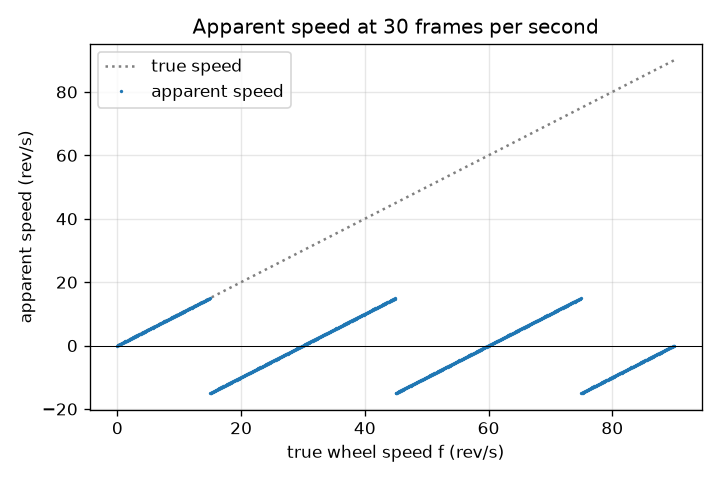
\includegraphics[width=0.85\linewidth]{figures/s01_apparent_vs_true.png}\\\small Apparent speed against true speed at 30 fps: a sawtooth that repeats every 30 rev/s.\end{center}

\subsection*{E. Worked example}
A wheel turns 28 rev/s and is filmed at 30 frames per second. How far does the marker turn between frames, what does the viewer see, and how fast does the wheel seem to go?
\begin{enumerate}[nosep]
\item Turn between frames: step = 360 x 28 / 30 = 336 degrees.
\item The viewer sees the shortest way: 336 degrees is the same place as 336 - 360 = -24 degrees, so the marker seems to move 24 degrees backwards each frame.
\item Apparent speed = -24 / 360 x 30 = -2 rev/s.
\item Check with f - k fs: k = round(28 / 30) = 1, so 28 - 30 = -2 rev/s. The two methods agree.
\end{enumerate}
\textbf{Answer.} The marker really turns 336 degrees per frame, but is seen to turn 24 degrees backwards: the wheel seems to go backwards at 2 rev/s.

\subsection*{F. Questions}
\begin{enumerate}[nosep]
\item \textbf{Conceptual.} A wheel turns slightly slower than fs rev/s (for example 29 rev/s at 30 fps). Why does it seem to turn slowly backwards, and not forward?
\item \textbf{Numerical.} A wheel turns 33 rev/s and is filmed at 24 frames per second. Find the turn per frame, the apparent turn and the apparent speed. Do a sanity check.
\item \textbf{Graph and simulation interpretation.} Using the sawtooth graph for 30 frames per second, for which true speeds between 0 and 60 rev/s does the wheel seem to go backwards, and where does it seem frozen?
\item \textbf{Design and optimisation challenge.} A wheel turns 29 rev/s. You may film with 24, 25, 28, 29, 30 or 60 frames per second. Which choice shows it turning slowly forward at no more than 1 rev/s? Which choice shows its true speed? What does the true-speed choice cost?
\end{enumerate}

\section{Session 2: The alias formula and the Nyquist limit}

\subsection*{A. Real-world problem}
A sound card, an oscilloscope and a camera all measure a continuous signal only at fixed instants. Session 1 found the sawtooth by looking at pictures. Engineers need a rule: if the fastest thing in the signal oscillates at f\_max hertz, how often must we measure so that no fast signal is mistaken for a slow one? And how do we know which slow signal a fast one will pose as? A table fan with four blades turns 12 rev/s: what frame rate shows it correctly?

\subsection*{B. Concept and theory}
Sampling a signal sin(2 pi f t) at the instants t\_n = n / fs gives the numbers x[n] = sin(2 pi f n / fs). If we replace f by f + k fs, where k is a whole number, the angle grows by 2 pi k n, a whole number of turns, and the samples do not change. So every frequency in the list ..., f - fs, f, f + fs, f + 2 fs, ... gives the same samples; and because sin(-a) = -sin(a) the negative of each gives the same samples up to a sign. Choose k = round(f / fs). Then f - k fs lies between -fs/2 and +fs/2 and is the smallest of the equivalent frequencies; its size is the alias frequency. It equals f for f below fs/2 and folds back (zigzags) above. The limit fs/2 is the Nyquist frequency. A signal whose highest frequency is f\_max is safe only if fs \textgreater{} 2 f\_max; exactly 2 f\_max is not enough (a sine sampled at its zero crossings gives all zeros). For a wheel with N identical blades or spokes, the picture repeats N times per turn, so the signal frequency is N f, not f; the apparent wheel speed is the signed alias of N f divided by N.

\begin{itemize}[nosep]
\item f: signal frequency (Hz)
\item fs: sampling rate (samples/s (Hz))
\item k: nearest whole number of sampling rates, round(f / fs) (no unit)
\item f\_alias: alias frequency, \textbar{}f - k fs\textbar{} (Hz)
\item f\_N: Nyquist frequency, fs / 2 (Hz)
\item N: number of identical blades or spokes (no unit)
\item f\_pattern: frequency of the repeating picture, N f (Hz)
\end{itemize}

\begin{equation*}
x[n]=\sin\!\left(2\pi f\,\frac{n}{f_s}\right)
\end{equation*}

\begin{equation*}
\sin\!\left(2\pi (f+k f_s)\frac{n}{f_s}\right)=\sin\!\left(2\pi f\frac{n}{f_s}+2\pi k n\right)=\sin\!\left(2\pi f\frac{n}{f_s}\right)
\end{equation*}

\begin{equation*}
f_{\text{alias}}=\left|f-k f_s\right|,\quad k=\mathrm{round}\!\left(\frac{f}{f_s}\right),\quad 0\le f_{\text{alias}}\le \frac{f_s}{2}
\end{equation*}

\begin{equation*}
f_s>2f_{\max}\quad\text{(Nyquist condition)},\qquad f_{\text{pattern}}=N f
\end{equation*}

\begin{center}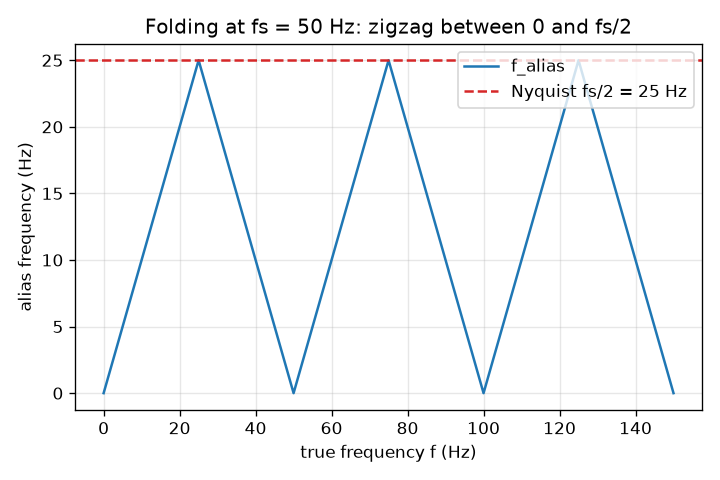
\includegraphics[width=0.85\linewidth]{figures/s02_folding.png}\\\small Alias frequency against true frequency at fs = 50 Hz, with the Nyquist limit at 25 Hz.\end{center}

\subsection*{E. Worked example}
A 40 Hz sine is sampled at 50 Hz. Find the alias frequency, the signed alias, and check with one sample.
\begin{enumerate}[nosep]
\item Nyquist frequency = 50 / 2 = 25 Hz. Since 40 Hz is above 25 Hz, aliasing will happen.
\item k = round(40 / 50) = round(0.8) = 1.
\item Signed alias = 40 - 1 x 50 = -10 Hz, so the alias frequency is 10 Hz.
\item Check with sample n = 1: x[1] = sin(2 pi x 40 / 50) = sin(2 pi x 0.8) = sin(288 degrees) = -0.951.
\item A -10 Hz sine gives sin(2 pi x (-10) / 50) = sin(-72 degrees) = -0.951. They match.
\end{enumerate}
\textbf{Answer.} The alias frequency is 10 Hz (signed -10 Hz); the 40 Hz samples are exactly those of a -10 Hz sine. The 40 Hz signal poses as a slow 10 Hz one.

\subsection*{F. Questions}
\begin{enumerate}[nosep]
\item \textbf{Conceptual.} After a signal has been sampled, can any processing of the samples tell a 40 Hz sine from its 10 Hz alias at fs = 50 Hz? Why is the only real cure a change before sampling?
\item \textbf{Numerical.} A 130 Hz signal is sampled at 100 Hz. Find the alias frequency and give two other frequencies that give the same samples.
\item \textbf{Graph and simulation interpretation.} On the folding graph for fs = 50 Hz, at which true frequencies from 0 to 150 Hz is the alias exactly 10 Hz?
\item \textbf{Design and optimisation challenge.} Design: a four-blade fan turns 12 rev/s. A phone can film at 30, 60, 100 or 120 frames per second. Which rates show the true speed and direction? What is the minimum, and what does a higher rate cost?
\end{enumerate}

\section{Session 3: Simulate, find the folded peak, recover the true speed}

\subsection*{A. Real-world problem}
You are handed two video clips of a fan, one filmed at 30 and one at 24 frames per second, and nothing else. In each the marked blade seems to turn backwards, slowly. The fan could be turning at almost any of an endless list of speeds. How do you find the real one, how sure can you be, and what do real cameras (blurry shutters, uneven timing) do to your measurement?

\subsection*{B. Concept and theory}
The FFT of N samples taken at rate fs lists the frequencies 0, fs/N, 2 fs/N, ..., fs/2; a pure sine appears as a peak at the alias frequency, so the peak position can be tested against the formula of Session 2 to within one bin, fs/N. A clip of a marker gives an apparent speed with a sign: each frame's marker angle is found, the steps between frames are folded into -180 to +180 degrees and averaged. One clip says f = a1 + k1 fs1 for a whole number k1; a second clip says f = a2 + k2 fs2. Only values that appear in both lists are possible. If both apparent speeds are signed, the pair repeats only after lcm(fs1, fs2) rev/s (whole-number rates), so the answer is unique below that limit; with the same rate twice, or a rate that is a multiple of the other, the limit stays small. If only the sizes \textbar{}a\textbar{} are known, we also have to try -a. Two real effects: timing jitter of standard deviation s turns the phase of every sample by a random amount 2 pi f s, which shrinks the coherent peak by exp(-(2 pi f s)\textasciicircum{}2 / 2); and a shutter open for tau seconds averages the signal over tau, multiplying a sine of frequency f by \textbar{}sinc(f tau)\textbar{}, sinc(x) = sin(pi x) / (pi x), a built-in low-pass filter that acts before sampling.

\begin{itemize}[nosep]
\item N: number of samples or frames (no unit)
\item fs: sampling or frame rate (Hz)
\item a1, a2: signed apparent speeds measured in clip 1 and 2 (rev/s)
\item k1, k2: unknown whole numbers (no unit)
\item L: unambiguous range, lcm(fs1, fs2) (rev/s)
\item s: standard deviation of timing jitter (s)
\item tau: exposure time (shutter open) (s)
\end{itemize}

\begin{equation*}
\Delta f_{\text{bin}}=\frac{f_s}{N}
\end{equation*}

\begin{equation*}
f=a_1+k_1f_{s1}=a_2+k_2f_{s2}
\end{equation*}

\begin{equation*}
L=\mathrm{lcm}(f_{s1},f_{s2})
\end{equation*}

\begin{equation*}
\frac{A_{\text{measured}}}{A}=e^{-\frac{1}{2}(2\pi f s)^2},\qquad \frac{A_{\text{exposed}}}{A}=\left|\frac{\sin(\pi f\tau)}{\pi f\tau}\right|
\end{equation*}

\begin{center}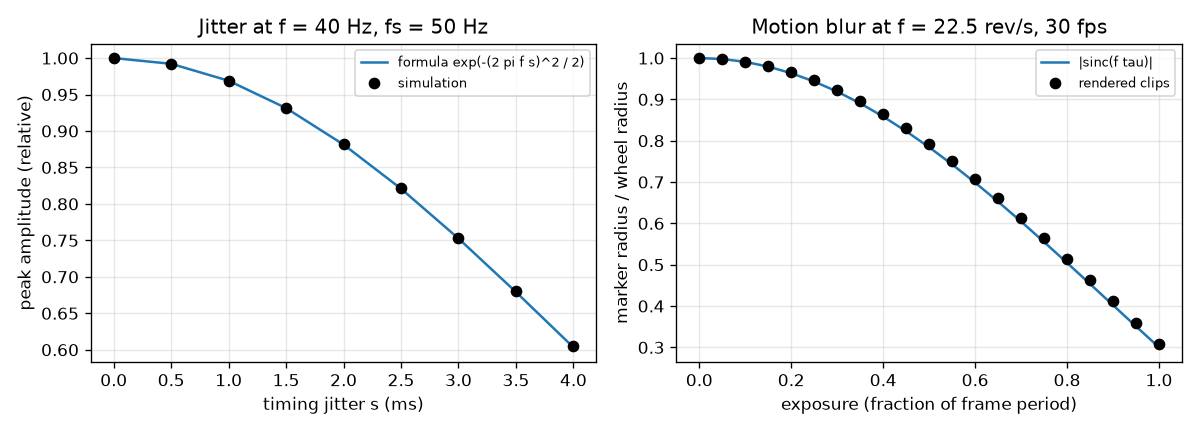
\includegraphics[width=0.85\linewidth]{figures/s03_jitter_exposure.png}\\\small Simulation against the jitter formula (left) and the exposure sinc formula (right).\end{center}

\subsection*{E. Worked example}
The 30 fps clip shows the marker at -7.5 rev/s and the 24 fps clip shows it at -1.5 rev/s. The fan turns at less than 60 rev/s. Find its true speed and say how sure you are.
\begin{enumerate}[nosep]
\item Clip 1 allows f = -7.5 + 30 k: ..., -7.5, 22.5, 52.5, 82.5, ...
\item Clip 2 allows f = -1.5 + 24 m: ..., -1.5, 22.5, 46.5, 70.5, ...
\item Values in both lists below 60: only 22.5 (k = 1 and m = 1). Check: -7.5 + 30 = 22.5 and -1.5 + 24 = 22.5.
\item Next common value: 22.5 + lcm(30, 24) = 22.5 + 120 = 142.5, far above the bound, so the answer is unique below 142.5 rev/s.
\item In rpm: 22.5 x 60 = 1350 rpm. Also check the simulation: sampled at 30 Hz the FFT peak is at 7.5 Hz, matching the formula.
\end{enumerate}
\textbf{Answer.} The fan turns 22.5 rev/s (1350 rpm), and this is the only possibility below 142.5 rev/s.

\subsection*{F. Questions}
\begin{enumerate}[nosep]
\item \textbf{Conceptual.} Why does a long exposure act as an anti-alias filter, and why can this not be repaired after the video is recorded?
\item \textbf{Numerical.} A frame clock has 1 millisecond of random timing jitter. By what factor does the peak of a 40 Hz signal shrink? Do the same for a 400 Hz signal. Which signal suffers more and why?
\item \textbf{Graph and simulation interpretation.} In the spectrum figure the FFT of the 22.5 Hz signal sampled at 30 Hz peaks at 7.5 Hz. Name four other true frequencies that would give a peak at the same place.
\item \textbf{Design and optimisation challenge.} Design: the first camera runs at 30 fps and fan speeds up to 100 rev/s must be recovered uniquely from signed measurements. Which second frame rate would you choose from 15, 20, 24, 25 and 60? Justify the choice.
\end{enumerate}

\section{Session 4: Noise-proof recovery of the true speed}

\subsection*{A. Real-world problem}
In Session 3 the apparent speeds were exact, and the true speed was the one number on both ladders. A real measurement is noisy: the marker is found a few pixels off, or the clip has only a few frames. With 0.3 rev/s of noise on both apparent speeds the Session 3 rule, which accepts two rungs closer than 0.3 rev/s, is right in only about half of the cases and gives no answer in the rest. How do we recover the true speed from numbers that are slightly wrong, and how sure can we be? This is general education about signal processing, not a measurement method for any safety decision.

\subsection*{B. Concept and theory}
A clip of $n$ frames gives $n$ marker angles, each wrong by $\sigma_\theta$ radians. The mean turn per frame telescopes, so the noise of the apparent speed is $\sigma=f_s\sqrt2\,\sigma_\theta/(2\pi(n-1))$ and falls like $1/(n-1)$. Instead of a yes/no tolerance, every pair of rungs $(c_1,c_2)$, one from each ladder, is scored by its gap $|c_1-c_2|$; the pair with the smallest gap gives the answer $\hat f=(c_1+c_2)/2$, the least-squares answer. The error of the middle has standard deviation $\sigma/\sqrt2$, which no rule can beat, and the chance of being within $t$ is $\mathrm{erf}(t/\sigma)$. A wrong pair wins only if $|n_1-n_2|$ exceeds half the gap between neighbouring pairs, $\gcd(f_{s1},f_{s2})/2$, which limits the noise a pair of rates survives.

\begin{equation*}
\hat f=\frac{c_1+c_2}{2},\qquad \mathrm{sd}(\hat f)=\frac{\sigma}{\sqrt2},\qquad P(|\hat f-f|\le t)=\operatorname{erf}\!\left(\frac{t}{\sigma}\right)
\end{equation*}

\begin{center}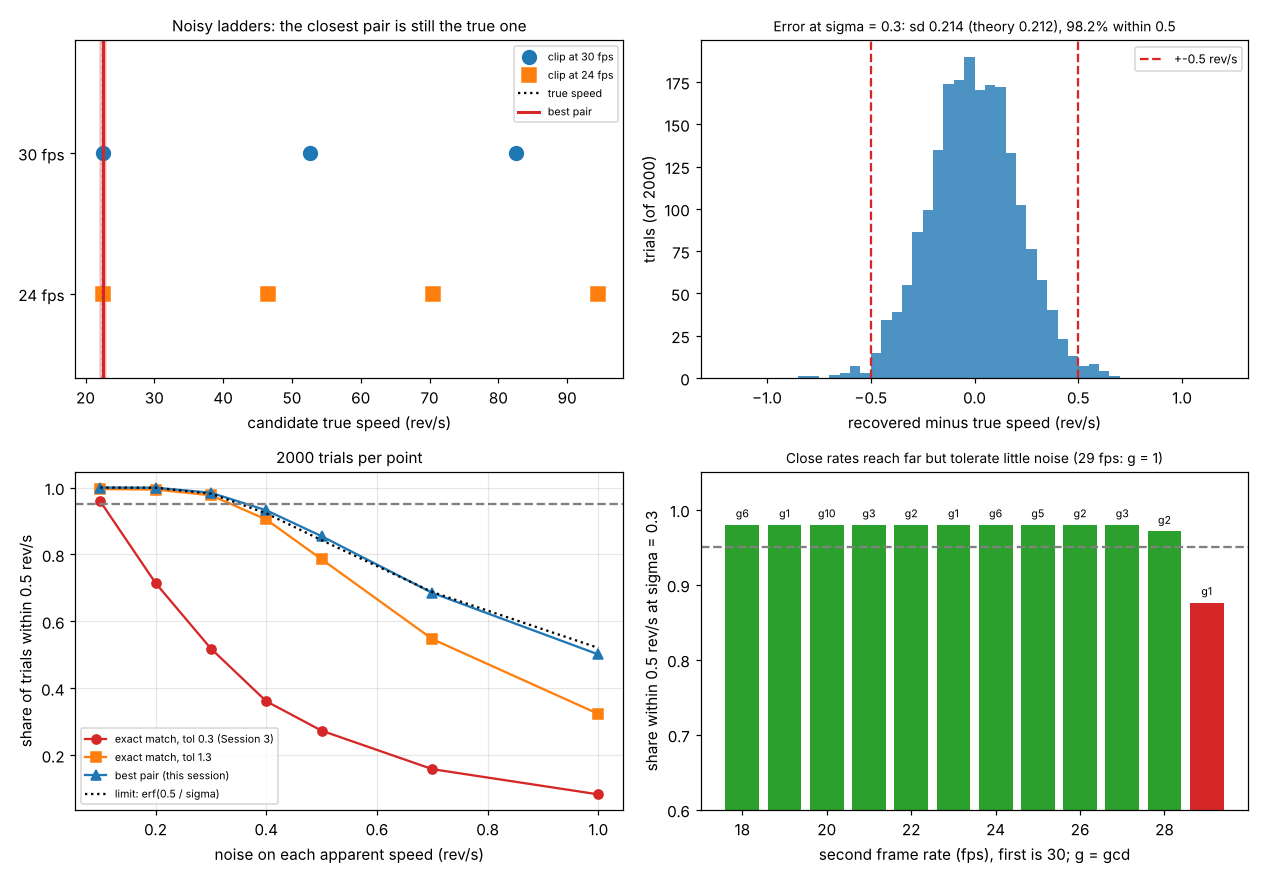
\includegraphics[width=0.85\linewidth]{figures/s04_noise_proof.png}\\\small One noisy trial with its ladders, the error of 2000 trials, the share right against noise for three rules, and the share right for second frame rates from 18 to 29 fps.\end{center}

\subsection*{E. Worked example}
Rates 30 and 24 fps, $\sigma=0.3$ rev/s, range 5 to 59 rev/s, measured apparent speeds $-7.2$ and $-1.8$ rev/s.
\begin{enumerate}[nosep]
\item Rungs: $-7.2+30k$ gives 22.8 and 52.8; $-1.8+24m$ gives 22.2 and 46.2.
\item Gaps: 0.6, 6.6, 23.4 and 30.6. The Session 3 rule needs 0.3 or less and gives no answer; the best pair is (22.8, 22.2).
\item The middle is 22.5 rev/s with uncertainty $0.3/\sqrt2=0.21$ rev/s; the margin is $(6.6-0.6)/(0.3\sqrt2)=14.1$.
\end{enumerate}
\textbf{Answer.} 22.5 $\pm$ 0.21 rev/s (1350 rpm).

\subsection*{F. Questions}
\begin{enumerate}[nosep]
\item \textbf{Conceptual.} The measurements are good to 0.3 rev/s and the Session 3 rule asks for a match within 0.3 rev/s. Why does it still fail about half of the time?
\item \textbf{Numerical.} Rates 30 and 25 fps, $\sigma=0.4$ rev/s, range 5 to 59 rev/s, measured apparent speeds 4.3 and 8.8 rev/s. Give the recovered speed with its uncertainty and margin, and say what the Session 3 rule does.
\item \textbf{Graph and simulation interpretation.} In the bottom left panel, at $\sigma=0.7$ the best pair is right in 68.5 percent of the trials, about the dotted limit, while the Session 3 rule is right in 16 percent. What does this tell you about the remaining failures?
\item \textbf{Design and optimisation challenge.} A marker is found with an error of 0.1 rad in each frame of a clip at 30 fps. How many frames are needed to be within 0.5 rev/s in at least 95 percent of the trials, and in at least 99 percent?
\end{enumerate}

\section{Session 5: A third clip: a wider range and less noise}

\subsection*{A. Real-world problem}
Two clips at 30 and 24 fps cannot tell 22.5 rev/s from 142.5, 262.5 or 382.5 rev/s: the pair of pictures repeats every $\mathrm{lcm}(30,24)=120$ rev/s. A turbine, a drill or a model engine can easily turn faster than that. A third clip at 25 fps stretches the range to 600 rev/s. Why does it work, which third frame rate helps and which does not, and what does the extra clip do to the noise? This is general education about signal processing, not a measurement method for any safety decision.

\subsection*{B. Concept and theory}
Each clip allows a ladder of rungs $a+kf_s$, and a speed on all the ladders fits every clip. A wrong speed $f'=f+d$ looks the same as $f$ on a clip at $f_s$ when $d$ is a whole number of frame rates, so it fools all three clips only when $d$ is a multiple of $\mathrm{lcm}(f_{s1},f_{s2},f_{s3})$: the unambiguous range is the least common multiple of all the rates. A third rate adds nothing when it divides the lcm of the other two (20, 24, 30, 40 and 60 fps next to 30 and 24), and a rate that helps can still be too small (36 fps gives 360). With noise, the best set of rungs, one per ladder, is the one whose members are closest to each other; its mean is the answer, with standard deviation $\sigma/\sqrt n$.

\begin{equation*}
f'=f+d\ \text{looks the same on all clips}\iff d=k\,\mathrm{lcm}(f_{s1},f_{s2},f_{s3}),\qquad P(|\hat f-f|\le t)=\operatorname{erf}\!\left(\frac{t\sqrt n}{\sigma\sqrt2}\right)
\end{equation*}

\begin{center}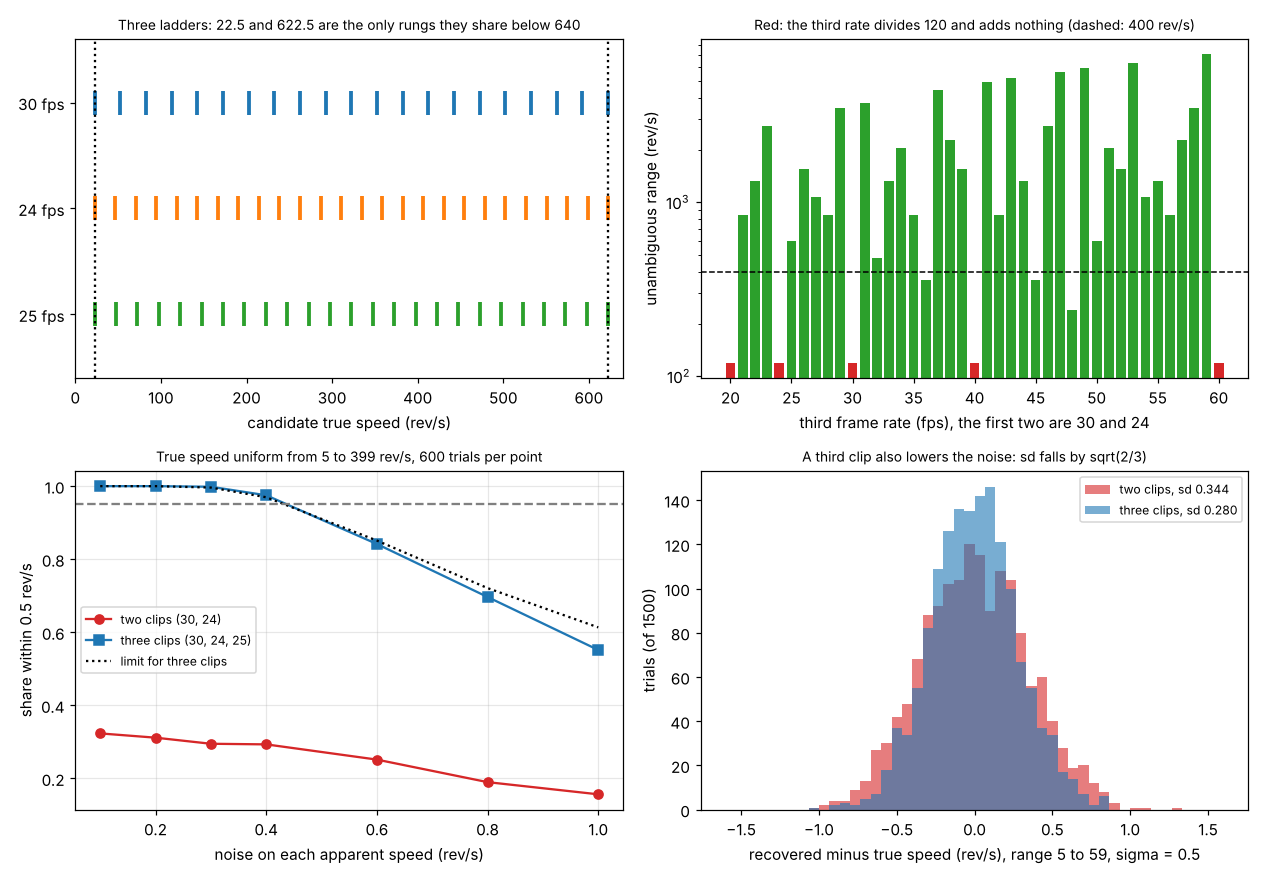
\includegraphics[width=0.85\linewidth]{figures/s05_third_clip.png}\\\small Three ladders, the range for every third rate, the share right against noise with two and three clips, and the error with two and three clips.\end{center}

\subsection*{E. Worked example}
Apparent speeds $-7.5$, $-1.5$ and $-2.5$ rev/s at 30, 24 and 25 fps.
\begin{enumerate}[nosep]
\item Clips 1 and 2 share 22.5, 142.5, 262.5 and 382.5 below 400 rev/s (120 apart).
\item Clip 3 allows $-2.5+25j$: 142.5, 262.5 and 382.5 are not on its ladder (145, 265 and 385 are not multiples of 25); only 22.5 is.
\item The next shared speed is $22.5+600=622.5$.
\end{enumerate}
\textbf{Answer.} Two clips leave 22.5, 142.5, 262.5 and 382.5; three clips leave only 22.5, unique up to 600 rev/s.

\subsection*{F. Questions}
\begin{enumerate}[nosep]
\item \textbf{Conceptual.} With 30 and 24 fps, a speed 120 rev/s above the true one fools both clips. Why does it no longer fool a third clip at 25 fps?
\item \textbf{Numerical.} The first two rates are 30 and 24 fps. For third rates of 20, 25, 36 and 40 fps give the range of the three rates, and say which make a fan of up to 400 rev/s recoverable.
\item \textbf{Graph and simulation interpretation.} In the top right panel the bars at 36, 45 and 48 fps are green but lie below the dashed 400 rev/s line. What does that mean for a fan at 380 rev/s filmed with 30, 24 and 45 fps?
\item \textbf{Design and optimisation challenge.} You have clips at 30 and 24 fps and must measure fans up to 400 rev/s with noise 0.3 rev/s. Which third rates in 20 to 60 fps work, which would you choose, and what share of trials will be within 0.5 rev/s?
\end{enumerate}

\section{Real-world mini-project}
\textbf{How fast does the fan really turn?.} A fan with one blade marked in red was filmed twice: once at 30 frames per second and once at 24 frames per second. At 30 fps the marker seems to turn backwards, at 24 fps it also seems to turn backwards but much more slowly. The clips are the function \texttt{mystery\_fan(fs)} of Session 3 (do not read the true speed from its code). The fan is known to turn at less than 60 revolutions per second. Measure both clips, recover the true speed, and confirm it with a third clip filmed at 25 fps.

\textbf{Recover the speed from noisy apparent speeds (classroom exercise only).} Given two noisy apparent speeds from a 30 and a 24 fps clip with noise 0.3 rev/s, return the most likely true speed and its uncertainty without using the true speed, then grade the rule on 2000 simulated trials. The Session 3 rule is right in 52 percent of the trials, exact matching with a tolerance of 1.3 in 97.7 percent, and the best pair in 98.5 percent, which meets the line of 95 percent within 0.5 rev/s and sits at the limit erf(0.5/0.3) = 98.2 percent. The 2 standard deviation band holds 95.2 percent of the errors. This is a teaching exercise on synthetic data, not a method for measuring a real machine.

\textbf{Choose three frame rates and recover a fast fan (classroom exercise only).} With clips at 30 and 24 fps and fans up to 400 rev/s, choose the third rate from 20 to 60 fps and check the choice by simulation. The rates 20, 24, 30, 36, 40, 45, 48 and 60 fps fail (their range stays at or below 400 rev/s) and the other 33 work; with 25 fps (range 600) the exact recovery is unique for all 1199 speeds tested, and with noise 0.3 rev/s the share within 0.5 rev/s is 99.9 percent with three clips against 28 percent with two. This is a teaching exercise on synthetic data, not a method for measuring a real machine.

\section{The path ahead}
\begin{enumerate}[nosep]
\item \textbf{Session 6: Fans with many identical blades.} A clip renderer and a measurement function for N identical blades, with one blade tinted to tell them apart.
\item \textbf{Session 7: A fan that spins up.} A tracker that follows the folded apparent speed through time and reconstructs the true speed curve.
\item \textbf{Session 8: Real cameras: variable frame rate and rolling shutter.} A simulator with frame timestamps from a clock with 0.5 percent jitter and a line-by-line shutter, plus a correction.
\end{enumerate}

\section{Answers and hints}

\subsection*{Session 1}
\begin{enumerate}[nosep]
\item \textbf{Conceptual.} Hint: Between two frames the marker turns almost one full turn. Compare it with a full turn. Solution: Between two frames the marker turns 348 degrees, which is 12 degrees short of a full turn. The eye ignores the full turn and sees the marker land 12 degrees before where it started, so it seems to move 12 degrees backwards per frame: -12 / 360 x 30 = -1 rev/s. A wheel slightly faster than fs would land slightly past its start and seem to move slowly forward.
\item \textbf{Numerical.} Hint: step = 360 f / fs, then fold into -180 to +180 degrees. Solution: step = 360 x 33 / 24 = 495 degrees. Folded: 495 - 360 = 135 degrees. Apparent speed = 135 / 360 x 24 = +9 rev/s (forward). Check: f - k fs with k = round(33 / 24) = round(1.375) = 1 gives 33 - 24 = 9 rev/s. Sanity: the apparent speed can never exceed fs / 2 = 12 rev/s in size, and 9 is below it.
\item \textbf{Graph and simulation interpretation.} Hint: Backwards means the curve is below zero. Solution: The curve is below zero for 15 \textless{} f \textless{} 30 rev/s and for 45 \textless{} f \textless{} 60 rev/s: backwards. It touches zero at f = 0, 30 and 60 rev/s: frozen. At exactly f = 15 and 45 rev/s the apparent speed is 15 in size, the flicker limit, and the direction cannot be told. Units: rev/s on both axes.
\item \textbf{Design and optimisation challenge.} Hint: Compute f - fs x round(f / fs) for each frame rate. Solution: The apparent speeds are +5 (24 fps), +4 (25 fps), +1 (28 fps), 0 (29 fps, frozen), -1 (30 fps, backwards) and +29 (60 fps). Only 28 fps shows slow forward motion of at most 1 rev/s. Only 60 fps shows the truth, because 60 is above twice 29 (Session 2 explains this rule). Trade-off: doubling the frame rate doubles the amount of data and needs more light per frame.
\end{enumerate}

\subsection*{Session 2}
\begin{enumerate}[nosep]
\item \textbf{Conceptual.} Hint: Look at the sample values you derived for the worked example. Solution: No. The samples of 40 Hz and -10 Hz are identical numbers, so no function of the samples can tell them apart. The information is lost at the instant of sampling. The cure must act before: sample faster (fs above 2 f\_max) or remove frequencies above fs/2 with a low-pass (anti-alias) filter first.
\item \textbf{Numerical.} Hint: k = round(130 / 100); then use f -/+ fs and the sign symmetry. Solution: k = round(1.3) = 1, so f\_alias = \textbar{}130 - 100\textbar{} = 30 Hz (signed +30). Frequencies with the same samples: 30 + 100 = 130, 30 - 100 = -70 (so 70 Hz up to a sign), 30 + 200 = 230, and the negatives. So 70 Hz and 170 Hz alias to 30 Hz as well. Sanity: 30 is between 0 and fs/2 = 50.
\item \textbf{Graph and simulation interpretation.} Hint: Draw a horizontal line at 10 Hz and read where it crosses the zigzag. Solution: The zigzag crosses 10 Hz at f = 10, 40, 60, 90, 110 and 140 Hz. They come in pairs symmetric about each multiple of 50: 50 -/+ 10, 100 -/+ 10, 150 - 10 (and 0 + 10).
\item \textbf{Design and optimisation challenge.} Hint: The picture repeats N f = 48 times per second. Apply the Nyquist condition to the pattern. Solution: The pattern frequency is 4 x 12 = 48 Hz, so fs must be above 2 x 48 = 96 frames per second: only 100 and 120 fps work (apparent +12 rev/s). At 30 fps the fan seems to turn at -3 rev/s (48 - 60 = -12 Hz, divided by 4) and at 60 fps also -3 rev/s. Exactly 96 would sit on the limit. A higher rate costs more data, more light per frame (shorter exposure) and storage; 100 fps is the cheapest choice with a margin of 4 percent only, 120 fps gives a safe margin of 25 percent.
\end{enumerate}

\subsection*{Session 3}
\begin{enumerate}[nosep]
\item \textbf{Conceptual.} Hint: Averaging a fast oscillation over a time much longer than one cycle gives about zero. Solution: During the exposure the sensor adds up the light, which averages the signal over tau seconds; a sine of frequency f is multiplied by \textbar{}sinc(f tau)\textbar{}, which is small once f tau is above 1. So fast motion is smeared away before the camera samples it and cannot fold. Afterwards the blur has already removed the information (a fully blurred marker has no position left), so no processing can bring it back.
\item \textbf{Numerical.} Hint: factor = exp(-(2 pi f s)\textasciicircum{}2 / 2). Solution: At 40 Hz: 2 pi x 40 x 0.001 = 0.2513, squared 0.0632, half 0.0316, factor exp(-0.0316) = 0.969, a loss of 3.1 percent. At 400 Hz: 2.513, squared 6.32, half 3.16, factor exp(-3.16) = 0.042, the peak is almost gone. The higher true frequency suffers more because the same timing error is a larger fraction of one cycle. It is the true frequency, not the alias, that counts.
\item \textbf{Graph and simulation interpretation.} Hint: The unsigned alias 7.5 Hz comes from f = 7.5 + 30 k and f = -7.5 + 30 k. Solution: 7.5 + 30 = 37.5, 22.5 (given), 52.5, 67.5, 82.5 and 7.5 itself. So the peak position alone cannot tell which one it was; a second frame rate is needed. The bin spacing here is 30 / 300 = 0.1 Hz, so the peak is read to about 0.05 Hz.
\item \textbf{Design and optimisation challenge.} Hint: The unique range is lcm(30, fs2); it must exceed 100. Solution: lcm(30, 15) = 30, lcm(30, 20) = 60 and lcm(30, 60) = 60 all fail (they are too small because the rates share large factors). lcm(30, 24) = 120 and lcm(30, 25) = 150 work. Choose 25 fps: the largest range (150 rev/s) gives margin if the true speed is a little above 100. Trade-off: the ladder rungs are spaced 30 and 25 rev/s apart, and the common rungs near each other differ by a few rev/s only when the rates are close, so measurement noise must stay below that difference; very close rates (such as 30 and 29) give a huge range but need very accurate measurements.
\end{enumerate}

\subsection*{Session 4}
\begin{enumerate}[nosep]
\item \textbf{Conceptual.} Hint: The rule compares the two rungs of the true pair with each other. How large is the difference of two noisy numbers? Solution: Each rung carries noise 0.3, so their difference has standard deviation $\sqrt2\times0.3=0.42$ rev/s. A tolerance of 0.3 is only 0.7 of that, so about 52 percent of the true pairs pass and the rest are rejected.
\item \textbf{Numerical.} Hint: Rungs are $4.3+30k$ and $8.8+25m$, searched 4 sigma beyond the range. Solution: Rungs 4.3, 34.3 and 8.8, 33.8, 58.8. The smallest gaps are 0.5 (middle 34.05) and 4.5. The speed is 34.05 $\pm$ 0.28 rev/s with margin $(4.5-0.5)/(0.4\sqrt2)=7.1$. The Session 3 rule needs a gap of 0.3 or less and gives no answer.
\item \textbf{Graph and simulation interpretation.} Hint: What is the standard deviation of the error of the best pair at sigma = 0.7? Solution: $0.7/\sqrt2=0.49$ rev/s, so 0.5 rev/s is about one standard deviation and erf(0.5/0.7) = 69 percent fall inside. The best pair chooses the right pair of rungs; the rest is the noise two numbers carry, and only a smaller sigma helps.
\item \textbf{Design and optimisation challenge.} Hint: $\sigma=f_s\sqrt2\sigma_\theta/(2\pi(n-1))$ and the share is erf(0.5/sigma). Solution: $\sigma=0.675/(n-1)$: n = 3 gives 0.338 and 96.4 percent; n = 4 gives 0.225 and 99.8 percent. Three frames for 95 percent, four for 99 percent.
\end{enumerate}

\subsection*{Session 5}
\begin{enumerate}[nosep]
\item \textbf{Conceptual.} Hint: When does adding $d$ rev/s to a speed leave a clip's apparent speed unchanged? Solution: When $d$ is a whole number of frame rates. $120=4\times30=5\times24$ fools clips 1 and 2, but $120/25=4.8$ is not whole, so clip 3 changes by $120-5\times25=-5$ rev/s. The first $d$ that works for all three is 600.
\item \textbf{Numerical.} Hint: The range is $\mathrm{lcm}(30,24,r)$ and $\mathrm{lcm}(30,24)=120$. Solution: 20 fps gives 120, 25 gives 600, 36 gives 360, 40 gives 120. Only 25 fps exceeds 400 rev/s.
\item \textbf{Graph and simulation interpretation.} Hint: What is $\mathrm{lcm}(30,24,45)$? Solution: 360 rev/s. $380=20+360$, so a fan at 380 rev/s looks exactly like one at 20 rev/s on all three clips and both fit. A rate that helps extends the range only to the new lcm.
\item \textbf{Design and optimisation challenge.} Hint: Use rate\_table(30, 24, range(20, 61)) and run\_trials. Solution: Every rate except 20, 24, 30, 36, 40, 45, 48 and 60 works (33 rates). At sigma = 0.3 the share within 0.5 rev/s is about 99.8 percent for 25, 26, 27, 29, 35 and 50 fps alike, so choose by practicality: 25 fps is a standard camera rate and its range of 600 covers the requirement.
\end{enumerate}

\section{How to join}
Read \texttt{CONTRIBUTING.md} in the repository, then pick an issue labelled \texttt{good first issue}. Repository: \url{https://github.com/KrunalPanchal1995/pan-iit-oss/tree/main/openalias}

\end{document}
